\section{Conceitos iniciais e sistemas de numeração}

\frame{
	\frametitle{Analógico x digital}
	\centering
	\scalebox{1.3}{
	

\tikzset{every picture/.style={line width=0.75pt}} %set default line width to 0.75pt        

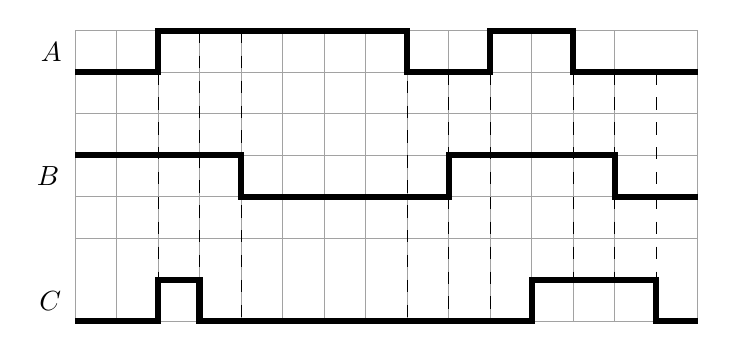
\begin{tikzpicture}[x=0.75pt,y=0.75pt,yscale=-1,xscale=1]
%uncomment if require: \path (0,300); %set diagram left start at 0, and has height of 300

%Shape: Grid [id:dp34531111101152123] 
\draw  [draw opacity=0] (100,40) -- (400,40) -- (400,180) -- (100,180) -- cycle ; \draw  [color={rgb, 255:red, 162; green, 162; blue, 162 }  ,draw opacity=1 ] (120,40) -- (120,180)(140,40) -- (140,180)(160,40) -- (160,180)(180,40) -- (180,180)(200,40) -- (200,180)(220,40) -- (220,180)(240,40) -- (240,180)(260,40) -- (260,180)(280,40) -- (280,180)(300,40) -- (300,180)(320,40) -- (320,180)(340,40) -- (340,180)(360,40) -- (360,180) ; \draw  [color={rgb, 255:red, 162; green, 162; blue, 162 }  ,draw opacity=1 ] (100,60) -- (400,60)(100,80) -- (400,80)(100,100) -- (400,100)(100,120) -- (400,120)(100,140) -- (400,140) ; \draw  [color={rgb, 255:red, 162; green, 162; blue, 162 }  ,draw opacity=1 ] (100,40) -- (400,40) -- (400,180) -- (100,180) -- cycle ;
%Straight Lines [id:da9908667716444586] 
\draw  [dash pattern={on 4.5pt off 4.5pt}]  (140,60) -- (140,160) ;


%Straight Lines [id:da9489034074703155] 
\draw  [dash pattern={on 4.5pt off 4.5pt}]  (160,40) -- (160,160) ;


%Straight Lines [id:da7444148673969375] 
\draw  [dash pattern={on 4.5pt off 4.5pt}]  (180,40) -- (180,180) ;


%Straight Lines [id:da33359589579811755] 
\draw  [dash pattern={on 4.5pt off 4.5pt}]  (260,40) -- (260,180) ;


%Straight Lines [id:da1689198722872045] 
\draw  [dash pattern={on 4.5pt off 4.5pt}]  (280,60) -- (280,180) ;


%Straight Lines [id:da2835936693187402] 
\draw  [dash pattern={on 4.5pt off 4.5pt}]  (300,60) -- (300,180) ;


%Straight Lines [id:da7069604701418795] 
\draw  [dash pattern={on 4.5pt off 4.5pt}]  (340,60) -- (340,160) ;


%Straight Lines [id:da35256438922338873] 
\draw  [dash pattern={on 4.5pt off 4.5pt}]  (360,60) -- (360,160) ;


%Straight Lines [id:da8396949759627998] 
\draw  [dash pattern={on 4.5pt off 4.5pt}]  (380,60) -- (380,160) ;


%Straight Lines [id:da8850959184881091] 
\draw [line width=2.25]    (100,60) -- (140,60) -- (140,40) -- (260,40) -- (260,60) -- (300,60) -- (300,40) -- (340,40) -- (340,60) -- (400,60) ;


%Straight Lines [id:da2574956876601695] 
\draw [line width=2.25]    (100,180) -- (140,180) -- (140,160) -- (160,160) -- (160,180) -- (320,180) -- (320,160) -- (380,160) -- (380,180) -- (400,180) ;


%Straight Lines [id:da8609754683162194] 
\draw [line width=2.25]    (100,100) -- (180,100) -- (180,120) -- (280,120) -- (280,100) -- (360,100) -- (360,120) -- (400,120) ;



% Text Node
\draw (88.5,50) node   {$A$};
% Text Node
\draw (87,110) node   {$B$};
% Text Node
\draw (88,170) node   {$C$};


\end{tikzpicture}
}
%	\centerline{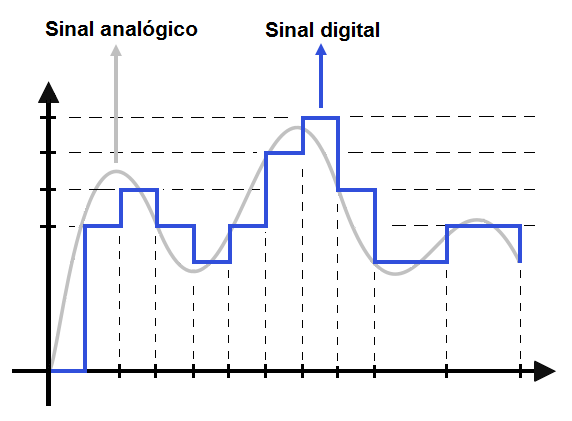
\includegraphics[width=0.7\linewidth]{Figuras/Ch1/analogdig.png}}
}

\frame{
	\frametitle{Analógico x digital}
	\centering
	\scalebox{0.8}{
		\deftkzbds
		
\begin{tikzpicture}[auto, node distance=2cm,>=Latex]
	% We start by placing the blocks
	\node [input] (input) {};
	\node [block, right=of input, xshift=0cm, align=center, text width=2cm] (computer) {$ h[n] $};
	\node [output, right =of computer] (output) {};
	\node [above, xshift=0.8cm] at (input) {$ x\left[n \right]  $};
	\node [above, xshift=-1cm] at (output) {$ y\left[n \right]  $};
	
	\draw [->] (input) -- (computer);
	\draw [->] (computer) -- (output);
\end{tikzpicture}}
%	\centerline{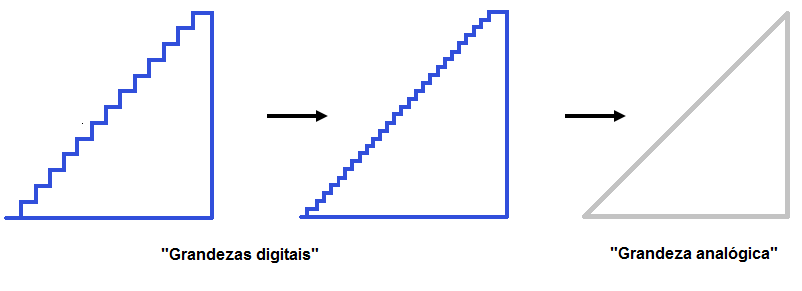
\includegraphics[width=0.8\linewidth]{Figuras/Ch1/rampaescada.png}}
}

\frame{
	\frametitle{Analógico x digital}
	\centerline{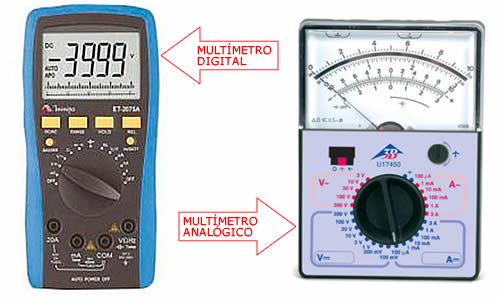
\includegraphics[width=0.7\linewidth]{Figuras/Ch1/multimetro.jpg}}
}

\frame{
	\frametitle{Vantagens e desvantagens}
	\begin{block}{Vantagens}
		\begin{itemize}
			\item Sistemas digitais são mais simples de serem projetados. 
			\item Maior facilidade em manter precisão e exatidão. 
			\item Operações podem ser programadas. 
			\item Menos afetados por ruídos.
			\item CI’s (Circuitos Integrados) podem ser fabricados com mais dispositivos.
		\end{itemize}
	\end{block}
}

\frame{
	\frametitle{Vantagens e desvantagens}
	\begin{block}{Desvantagens}
		\begin{itemize}
			\item O mundo é quase todo analógico. 
			\item Processar sinais digitais demanda tempo.
		\end{itemize}
	\end{block}
}

\frame{
	\frametitle{E no mundo real?}
	\begin{block}{Importante}
		Como converter?
	\end{block}

	\vspace{0.5cm}
	
	\centerline{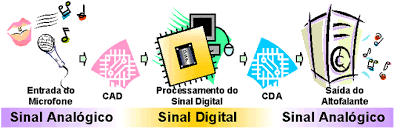
\includegraphics[width=0.8\linewidth]{Figuras/Ch1/mundoreal.png}}
}

\frame{
	\frametitle{Sistemas de numeração}
	\begin{block}{As quatro bases numéricas}
		\begin{itemize}
			\item Decimal
			\item Binário
			\item Octal
			\item Hexadecimal
		\end{itemize}
	\end{block}
}

\frame{
	\frametitle{Sistemas de numeração}
	\begin{block}{Sistema decimal}
		\begin{itemize}
			\item Caracteres 0 a 9.
			\item Notação posicional -- base 10.
			\item MSB x LSB.
			\item Exemplos de representação.
		\end{itemize}
	\end{block}

	\vspace{0.3cm}
	\centerline{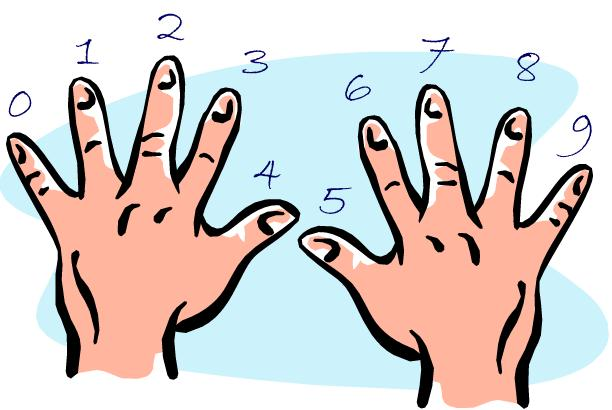
\includegraphics[width=0.5\linewidth]{Figuras/Ch1/decimal.jpg}}
}

\frame{
	\frametitle{Sistemas de numeração}
	\begin{block}{Sistema binário}
		\begin{itemize}
			\item 2 dígitos.
			\item Notação posicional -- base 2.
			\item MSB x LSB.
			\item Quantidade de dígitos para representar -- como?.
		\end{itemize}
	\end{block}

	\vspace{0.3cm}
	
	\centerline{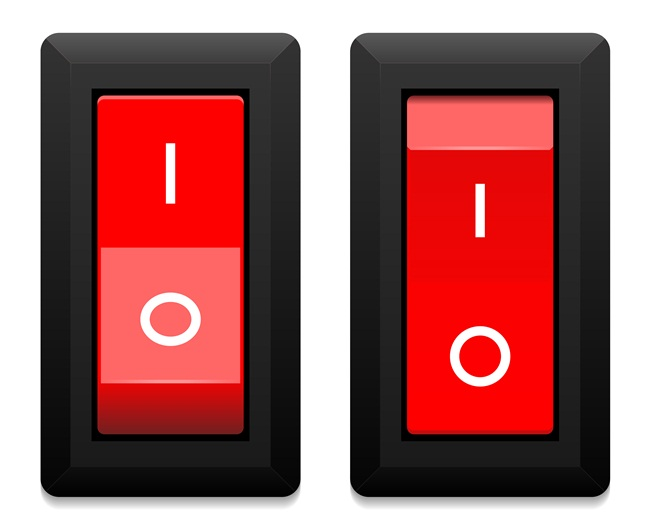
\includegraphics[width=0.4\linewidth]{Figuras/Ch1/binario.jpg}}
}

\frame{
	\frametitle{Sistemas de numeração}
\begin{block}{Tipos de dados binários}
%	\renewcommand{\arraystretch}{1.2}
	\centering
	\resizebox{\textwidth}{!}{
		\begin{tabular}{p{8em}C{8em}}
			\toprule
			\thead{\normalsize Tipo de dado} & \text{\thead{\normalsize Tamanho \\ 
				\normalsize (em bits)}} \\ \midrule
			bit & 1 \\
			nibble & 4 \\
			byte & 8 \\
			word & 16 \\
			double word & 32 \\
			\bottomrule
		\end{tabular}
	}
	\end{block}
}

\frame{
	\frametitle{Aritmética binária}
	\begin{block}{Adição}
			
		\begin{equation*}
		\mathlarger{\mathlarger{\mathlarger{
			\begin{array}{@{}B1}
				00\carry 11 \\
				{} + 0101 \\ \hline
				0110 \\
			\end{array}}}}
		\end{equation*}
	\end{block}
}

\frame{
	\frametitle{Aritmética binária}
	\begin{block}{Subtração}
		
		\begin{equation*}
		\mathlarger{\mathlarger{\mathlarger{
					\begin{array}{@{}B2}
						1\tikzmark{p1} & \carry1\tikzmark{p2}\carry 011 \\
					{}-	0 	& 1101 \\ \hline
						0 	& 1110 \\
					\end{array}}}}
		\end{equation*}
		
		\begin{tikzpicture}[overlay,remember picture]
			\draw (p1) ++(6,5.1) -- +(0.2,0.5);
			\draw (p1) ++(6.35,5.1) -- +(0.2,0.5);
		\end{tikzpicture}
	\end{block}
}

\frame{
	\frametitle{Aritmética binária}
	\begin{block}{Multiplicação}
		\centering
		\binmult{5}{6}
	\end{block}
%		\centerline{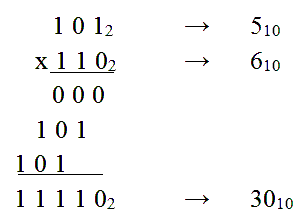
\includegraphics[width=0.5\linewidth]{Figuras/Ch1/multbin.png}}
}


\section*{Conversão entre bases numéricas}

\frame{
	\frametitle{Conversão binário-decimal}
	\begin{block}{Procedimento}
		\begin{itemize}
			\item Se dá pela soma das multiplicações de cada termo por sua potência de base 2 equivalente.
		\end{itemize}
	
		\centering
		\ConvertFromBase{2}{11001}
	\end{block}
%	\centerline{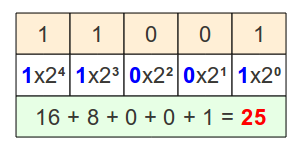
\includegraphics[width=0.5\linewidth]{Figuras/Ch1/bindec.png}}
}

\frame{
	\frametitle{Conversão decimal-binário}
	\begin{block}{Procedimento}
		\begin{itemize}
			\item Método das divisões sucessivas 
		\end{itemize}
	
		\vspace{0.5cm}
	
		\centering
		\begin{tabular}{c}
			\basetenconversiontable{12}{2}
		\end{tabular}
	\end{block}
%	\centerline{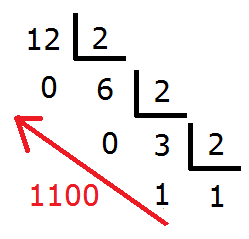
\includegraphics[width=0.5\linewidth]{Figuras/Ch1/decbin.png}}
}

\frame{
	\frametitle{Conversão fração decimal-binário}
	\begin{block}{Procedimento}
		\begin{itemize}
			\item Método das multiplicações sucessivas
		\end{itemize}
	
		\vspace{0.5cm}
		
		\ConvertitEnBaseB{3.75}{2}
	\end{block}
}

\section*{Exercícios}

\frame{
	\frametitle{Exercícios}

	\begin{block}{}
		01. Converter os seguintes números binários para decimais:

		\begin{itemize}
			\item \num{11111}$ _2 $
			\item \num{1001100}$ _2 $
			\item \num{1011,11}$ _2 $
			\item \num{1100,0011}$ _2 $
		\end{itemize}

		02. Converter os seguintes números decimais para binários:

		\begin{itemize}
			\item \num{215}
			\item \num{102}
			\item \num{9,92}
			\item \num{7,47}
		\end{itemize}
	\end{block}
}

\section*{Referências}

\frame{
	\frametitle{Referências e exercícios complementares}
	\begin{itemize}
		\item IDOETA, Ivan V. e CAPUANO, Francisco G. Elementos de Eletrônica Digital. São Paulo: Editora Érica, ed. 40. 2008.
	\end{itemize}

	\centering{\alert{Página 36 - \textbf{1.6.1 até 1.6.5, 1.6.17 até 1.6.19}}}
}